% ==========================================================
\section{Feature Modeling}
\label{sec:feature-modeling}
% ==========================================================

Feature modeling provides a structured way to describe commonalities and variabilities within a family of related systems.
It is central to this thesis because the proposed graphical extensions build on feature models to represent both static product structure and runtime-relevant variation.
The following subsections introduce the background of Software Product Lines, explain how feature trees encode relationships between features, and outline how \gls{uvl} captures these ideas in a textual syntax.

% ----------------------------------------------------------
\subsection{Software Product Lines}
\label{subsec:spl}
% ----------------------------------------------------------

\gls{spl} shift development from isolated systems to a reuse-oriented engineering approach~\cite{clements_software_2002}.
The core idea is to build a shared asset base that can be systematically reconfigured into a family of related products tailored to specific market needs~\cite{lee_concepts_2002}.
By managing commonality and variability across the portfolio, organizations can reduce development costs and shorten time-to-market~\cite{pohl_software_2005}.
The process is typically divided into domain engineering and application engineering~\cite{buhne_modelling_2005, apel_overview_2009}.
During domain engineering, the focus lies on defining the relevant features and constraints that characterize the product family.
Application engineering then uses this model to derive specific products tailored to individual stakeholder requirements.

\gls{dspl} extend these traditional \gls{spl} concepts by integrating both static variability in space and dynamic variability over time into a unified framework~\cite{burdek_staged_2014}.
Rather than completely shifting variability resolution away from design time, \glspl{dspl} support multiple binding times to handle features across different operational modes~\cite{capilla_overview_2014}.
This approach allows developers to clearly distinguish between static features that are finalized prior to product derivation and dynamic features that remain open as variation points.
These enable autonomous system adaptation and reconfiguration at runtime.
To manage this increased complexity and temporal dependency, developers use extended feature models that assign binding times to specific features.

Feature models in general define the boundaries of what can be built and provide a structured view of product variation, making them a natural tool for managing this variability.

% ----------------------------------------------------------
\subsection{Feature Trees}
\label{subsec:feature-trees}
% ----------------------------------------------------------

\gls{foda} established the foundation for hierarchical decomposition by defining features as user-visible characteristics identified through rigorous domain analysis~\cite{kang_feature-oriented_1990}.
A feature model consists of a hierarchically arranged collection of features.
Its structural integrity relies on the relationships between parent and child features~\cite{kang_feature-oriented_1990, czarnecki_formalizing_2005}.

Across the literature~\cite{lee_concepts_2002, czarnecki_formalizing_2005, czarnecki_staged_2004, benavides_automated_2005, benavides_automated_2010}, basic feature models contain the following relationship types:

\begin{itemize}
    \item \textbf{Mandatory.}
    A child feature has a \textit{mandatory} relationship with its parent feature if the child is part of all products in which the parent is included.
    \item \textbf{Optional.}
    A child feature has an \textit{optional} relationship with its parent feature if the child is optionally part of all products in which the parent is included.
    \item \textbf{Or.}
    A set of child features has an \textit{or} relationship with their parent feature when at least one child is active in products where the parent is included.
    \item \textbf{Alternative.}
    A set of child features has an \textit{alternative} relationship with their parent feature when exactly one child is active in products where the parent is included.
    In other literature~\cite{lee_concepts_2002, benavides_automated_2005}, the \textit{alternative} relation can be combined with \textit{mandatory} or \textit{optional}, which allows for a selection of zero elements as well.
\end{itemize}

\begin{figure}
	\centering
	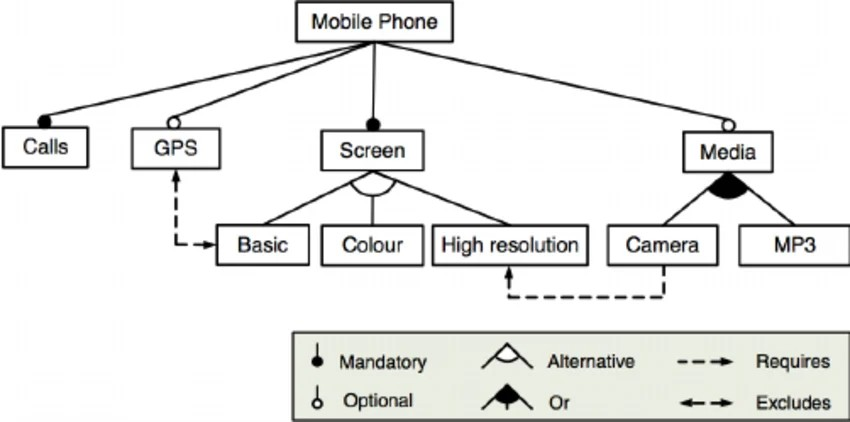
\includegraphics[width=\textwidth]{figures/feature-model.jpg}
	\caption[Example of Feature Model]{Example of a feature tree for a mobile phone, including cross-tree constraints. Taken from \cite{benavides_automated_2010}.}
    \label{fig:mobile_phone_feature_tree}
\end{figure}

Beyond these parent-child relationships, feature models may contain cross-tree constraints between features.
Typical examples are \textit{requires} and \textit{excludes}~\cite{galindo_automated_2019}.
A \textit{requires} constraint enforces that selecting one feature also requires selecting another.
An \textit{excludes} constraint stipulates that two features cannot be included in the same configuration.
More expressive formulations are also possible, including propositional constraints such as \texttt{A implies not B or not C}.
Figure~\ref{fig:mobile_phone_feature_tree} illustrates a feature tree with such cross-tree constraints.

% ----------------------------------------------------------
\subsection{Advancements to Feature Trees}
\label{subsec:advancements-to-feature-trees}
% ----------------------------------------------------------

Advanced feature modeling extends the traditional binary logic of \gls{foda} by introducing quantitative constraints and metadata.
These extensions support more complex configurations and more detailed resource tracking.

% ----------------------------------------------------------
\subsubsection{Cardinality-Based Modeling}
\label{subsubsec:cardinality-based-modeling}
% ----------------------------------------------------------

This approach borrows from \gls{uml} multiplicities to define how often and how many instances of a feature may appear in a configuration.

\textbf{Feature cardinality.}
A feature cardinality is assigned an interval $[n \dots m]$, where $n$ is the minimum and $m$ is the maximum number of instances permitted.
This generalizes traditional relationships:
\begin{itemize}
    \item Mandatory: $[1 \dots 1]$
    \item Optional: $[0 \dots 1]$
    \item Clones: Any range where $m > 1$, allowing multiple distinct instances of the same feature.
\end{itemize}

\textbf{Group cardinality.}
This restricts the selection of child features when a parent is active.
Represented by the interval $[n \dots n]$, it dictates that at least $n$ and at most $m$ children must be chosen.
This generalizes traditional relationships:
\begin{itemize}
    \item Alternative: $[1 \dots 1]$
    \item Or-Relationship: $[1 \dots k]$, where $k$ is the total number of available sub-features.
\end{itemize}

% ----------------------------------------------------------
\subsubsection{Attribute-Based Modeling}
\label{subsubsec:attribute-based-modeling}
% ----------------------------------------------------------

Attribute-based modeling extends standard feature models by attaching additional information to features in the form of attributes.
These extended models are often referred to as extended, advanced, or attribute-based feature models.
When the basic tree structure is not expressive enough, attributes provide a way to capture richer feature-specific information and support more advanced analyses.

Attributes are typically represented as key-value pairs and are commonly described by at least a name, a type, a domain, and a value.
Depending on the model, an attribute may store a numeric quantity, a boolean flag, or a string value.
Common examples include a feature's cost, memory consumption, or an associated URL.

Attributes are useful as metadata containers for tool-specific information or for values that should remain directly attached to a feature in the model structure.
They also enable metric computation, such as calculating the total price of a selected configuration, by aggregating attribute values across all chosen features.
In addition, attribute-based models support constraints over numeric and textual domains, enabling rules such as budget limits or consistency checks on string values.
This makes attributes a practical extension when propositional feature constraints alone are insufficient.

% ----------------------------------------------------------
\subsection{Universal Variability Language}
\label{subsec:universal-variability-language}
% ----------------------------------------------------------

The \glsentrylong{uvl} emerged to standardize these concepts into a unified textual exchange format, reducing fragmentation across modeling tools~\cite{sundermann_integration_2021, sundermann_yet_2021}. 
Designed for both human readability and automated processing, \gls{uvl} uses indentation-based nesting to represent the tree hierarchy and provides a dedicated block for cross-tree constraints. 

To balance simplicity with expressiveness, \gls{uvl} features an extensible design structured into three major language levels: Boolean, Arithmetic, and Type~\cite{sundermann_yet_2021}. 
The Boolean level acts as the core language, which is easily encoded as a SAT problem.
The Arithmetic and Type levels introduce numeric constraints and typed features that require more complex reasoning engines like SMT solvers. 
Additionally, \gls{uvl} includes optional minor levels to support advanced constructs such as feature cardinalities, group cardinalities, and string constraints.

To address the complexity of large-scale industrial product lines, \gls{uvl} incorporates an import mechanism that decomposes massive feature models into smaller, manageable sub-models~\cite{sundermann_yet_2021}. 
These sub-models can be maintained independently and composed into an overall model, using a namespace syntax similar to Java imports. 
Because of its standardized, extensible architecture, \gls{uvl} has been successfully integrated as a pivot language in various variability modeling and transformation frameworks, such as FeatureIDE, flamapy, and TraVarT~\cite{sundermann_integration_2021}.

In this thesis, \gls{uvl} serves as the foundational abstract syntax on which the proposed graphical extensions are mapped.
Listing~\ref{lst:mobile_phone_uvl} shows the \gls{uvl} representation of the same mobile phone example introduced in Figure~\ref{fig:mobile_phone_feature_tree}.
It is a direct textual encoding of that feature tree, including its hierarchy and cross-tree constraints.

\lstinputlisting[
    language=UVL, 
    float,
    floatplacement=ht,
    caption={[Mobile Phone UVL]UVL specification of the mobile phone feature model shown in Figure~\ref{fig:mobile_phone_feature_tree}}, 
    label={lst:mobile_phone_uvl}
]{code/feature-model.uvl}